\chapter{Sensors and Measurements}\label{chapter:sensors}

\textbf{Author: Lukas Leskovar} 

The means of perceiving ones surrounding environment are a crucial part of any robotic system. This chapter aims to describe the need for interoceptive measurements aiding the different algorithms used within Autumn as well as any sensory equipment supporting such data acquisition. To this end, the underlying principles and concepts behind the measurement techniques are illustrated.

\section{Motion Models}
Kinematic models in robotics are used for describing and planning state-transitions between consecutive robot poses. While Chapter \ref{chapter:slam} focuses on the theoretic basics of such models and how to build upon them, this section is going to focus on the practical concepts used in robot localization. To this end, classical odometry and velocity-based motion models are described.

To facilitate any equations later in this section, the robot's pose is described by its state vector 
\[
\begin{pmatrix}
	x \\
	y \\
	\theta \\
\end{pmatrix}
\] 
which defines its position as Cartesian coordinates and bearing as angular orientation $\theta$ in 2-dimensional space. 

\subsection{Odometry}
Ben-Ari and Mondada define this topic as follows: "Odometry—the measurement of distance—is a fundamental method used by robots for navigation.". \footcite[Page 69]{ben2017elements} 
When performing linear odometry, e.g. without considering orientation changes, this distance is calculated rather trivially by inferring it through measured time elapsed and the robot's velocity proportionally to the motor power. 
Other systems utilize wheel encoders to count the number of wheel rotations, thus allowing for a rather precise estimation of distance. 

With non-linear motion, the distances $d_{l}$ and $d_{r}$ moved by the left and right wheel are unequal, which requires the calculation of both updated position and bearing of the robot. 
Lets suppose a robot moved from position $\begin{pmatrix} x & y & \theta \end{pmatrix}^{T}$ to $\begin{pmatrix} x' & y' & \theta' \end{pmatrix}^{T}$ with a slight left turn caused by the right wheel turning faster than the left one. 
This scenario is depicted in Figure \ref{fig:odom} with $\varphi$ corresponding to the turn angle in radians, the radii $r_{l}, r_{c}, r_{r}$ describing the distance from the new position of the wheels and centre to point $P$, the origin of the turn. 

For small angles, these radii are approximately the same length as the distances $d_{l}, d_{c}$ and $d_{r}$, which allows for the turn angle to be calculated as follows:
\begin{align*}
	\varphi &= \frac{d_{i}}{r_{i}}, & i &= l, r, c  
\end{align*}

However, in practical scenarios where these radii and the point P are unknown, $\varphi$ has to be calculated only using $d_{l}$, $d_{r}$ and $b$, which corresponds to the distance between both robot wheels.

\begin{equation*}
	\begin{split}
		\varphi r_{r} = d_{r} \\
		\varphi r_{l} = d_{l} \\
		\varphi r_{r} - \varphi r_{l} = d_{r} - d_{l} \\
		\varphi = \frac{d_{r} - d_{l}}{r_{r} - r_{l}} \\ 
		\varphi = \frac{d_{r} - d_{l}}{b} \\
	\end{split}
\end{equation*}

To calculate the new coordinate positions the distance $d_{c}$ is computed:
\begin{equation*}
	d_{c} = \frac{d_{l} + d_{r}}{2}
\end{equation*}

The final pose is calculated as follows:

\begin{equation*}
	\begin{pmatrix}
		x' \\ 
		y' \\
		\theta'
	\end{pmatrix}
	= 
	\begin{pmatrix}
		-d_{c} \sin \varphi \\
		d_{c} \cos \varphi \\ 
		\theta + \varphi
	\end{pmatrix}
\end{equation*}

Because the assumptions above only apply for small distances, such computations should be performed continuously in any real-world system. However, due to uncertain measurements, these calculations inherit some margin of error integrated up over multiple iterations, thus causing a slight drift in the output.\footcite[Pages 69 - 77]{ben2017elements} 
This drift can be corrected using techniques discussed in Chapter \ref{chapter:slam}.

\begin{figure}
	\centering
	\includesvg[width=0.8\linewidth]{img/svg/odom}
	\caption{
		This diagram shows the geometry of how a slight turning motion can be calculated only using the distances $d_{l}$, $d_{r}$ and wheel offset $b$.
		The robot pose 
		$
			\begin{pmatrix}
				x &
				y &
				\theta 
			\end{pmatrix}^{T}
		$
		is associated with the center of the robot \footcite{ben2017elements}.
	}
	\label{fig:odom}
\end{figure}


\subsection{Inertial Measurement}
Another way of modelling motion usually utilized when a robot is not equipped with wheel encoders or wheels is based on the vehicle's velocities. Typically the inputs of velocity-based motion models are measured using Inertial Measurement Units (IMU), Gyroscopes and Accelerometers. 

The variables $v$ and $\omega$ denote the linear and angular velocities and are referred to as controls for the system. 
In contrast to odometry, which can only be calculated after a movement has been performed, these controls allow for prior motion planning. \footcite[Pages 92 - 99]{thrun2002probabilisticRobotics}

If these velocities stay fixed for the entire duration $\Delta t$ of the motion from 
$\begin{pmatrix} x & y & \theta \end{pmatrix}^{T}$
to
$\begin{pmatrix} x' & y' & \theta' \end{pmatrix}^{T}$
the robot moves in a circle with radius $r$ as seen in Figure \ref{fig:inertial}. The center $P$ of this circle with coordinates 
$
\begin{pmatrix}
	x_{P} & y_{P}
\end{pmatrix}
^{T}
$
can be evaluated as follows:

\begin{equation}
	\begin{split}
		x_{P} = x - \frac{v}{\omega} \sin \theta \\
		y_{P} = y + \frac{v}{\omega} \cos \theta
	\end{split}
\end{equation}

This allows for the new position to be calculated: 

\begin{equation}
	\begin{pmatrix}
		x' \\
		y' \\
		\theta'
	\end{pmatrix}
	=
	\begin{pmatrix}
		x_{P} + \frac{v}{\omega} \sin(\theta + \omega \Delta t) \\
		y_{P} - \frac{v}{\omega} \cos(\theta + \omega \Delta t) \\
		\theta + \omega \Delta t
	\end{pmatrix}
\end{equation}

Despite being incapable of calculating movements in advance, odometry should be preferred over velocity motion models as they pose higher localization accuracy. \footcite[Page 107]{thrun2002probabilisticRobotics}

\begin{figure}
	\centering
	\includesvg[width=0.5\linewidth]{img/svg/inertial}
	\caption{
		In this diagram, a slight turning motion of the robot is described by the translational velocity $v$ and angular velocity $\omega$. These velocities, if remaining unchanged, render the robot to move in a perfect circle with the centre point $P$ and radius $r = | \frac{v}{\omega}|$. Even if the angular velocity remains 0, the motion is still described as a circle with an infinite radius. \footcite[Pages 95 - 107]{thrun2002probabilisticRobotics}
	}
	\label{fig:inertial}
\end{figure}



\section{Depth Sensing}
Similar to motion models contributing to robot localization in Autumn, Depth-Sensing is utilized to perceive and map the drone's environment. 
The technologies in this section focus on mapping distance information to each point in the camera's field of view, thus providing 3D-Imaging.

\subsection{Structured Light}
One approach uses active illumination to project a varying intensity pattern onto the perceived scene, thus allowing a camera to extract 3D information from the distorted pattern as the scene's surface is non-planar. \footcite{geng2011StructuredLight}

\subsection{Time-of-Flight}
Time-of-Flight (ToF) sensors perform active triangulation, which is performed by emitting modulated light to be reflected by a scene, as described in Figure \ref{fig:activeTriangulation}. The distance to the scene is determined using the time difference between emission and detection of singular rays (more prominent with ToF Laser-Scanners like LiDAR) or the phase shift of light reflected by the whole scene. The latter allows for mapping depth information to the entire Field-of-View (FoV). 
%It may be necessary to differentiate mapping using depth perception sensors from LiDAR technologies which pose an alternative solution. 
Although LiDAR sensors fall under the category of ToF sensors, they perceive the distance to an object using pulsed lasers, thus outputting
the distance to singular points in the sensor's surroundings rather than depth information mapped to an image. \footcite{gokturk2004time} \footcite{velodyne2021LiDAR}
% LiDAR verwenden die Zeitdifferenz und berechnen mittels Trigonometrie die Distanz
As 3D-LiDAR sensors applied in many commercial mapping solutions are very expensive, they disqualify for use in Autumn. Instead, the project focuses on performing with approximate precision using relatively inexpensive camera-based equipment. 

\begin{figure}
	\centering
	\includesvg[width=0.8\linewidth]{img/svg/activeTriangulation}
	\caption{
		This diagram depicts a ToF depth camera emitting IR-light (red) onto a surface. The camera sensor then utilizes the phase-shift $\varphi$ between the emitted (red) and received signal (blue) to calculate the distance between the scene and sensor. \footcite{altuntas2021triangulation}
		% noch mehr schreiben
	}
	\label{fig:activeTriangulation}
\end{figure}


\subsection{Stereo Vision}
The last and most significant approach to Autumn performs passive triangulation using two cameras setup as seen in Figure \ref{fig:passiveTriangulation}. Although this eliminates the need for any light to be emitted, the problem of correspondence is introduced. Which deals with associating the different projections to the same point in the real world\footcite{ng2019StereoCorrespondence}. There are multiple approaches to this problem which are generally divided into global and local matching methods, with the latter being more computationally efficient while sacrificing quality. \footcite{do2019review}

In Autumn, this approach was pursued using a Stereolabs ZED 2i depth camera as it was superior to any competitors such as the Microsoft Kinect or Intel Realsense concerning availability and cost-effectiveness. 

\begin{figure}
	\centering
	\includesvg[width=0.8\linewidth]{img/svg/PassiveTriangulation}
	\caption{
		This diagram describes the camera setup found in passive triangulation systems. Using stereo-photogrammetry the distance to the perceived scene is calculated.\footcite{altuntas2021triangulation}
	}
	\label{fig:passiveTriangulation}
\end{figure}

\subsection{ZED 1 vs ZED 2i}
%As mentioned in Chapter \ref{chapter:architecture} the Stereolabs ZED 1 was used in a first prototype and later replaced with a 
Chapter \ref{chapter:architecture} mentions that the Stereolabs ZED 1 used in early prototypes was quickly replaced with the ZED 2i. This change was due to processing limitations and additional features provided by the newer product version.
This section aims to benchmark the two cameras from a depth-performance standpoint to review if the upgrade enhanced depth perception, thus improving the system output or if no changes were necessary when only considering depth-perception.

\subsubsection{Experiment}

\begin{figure}
	\centering
	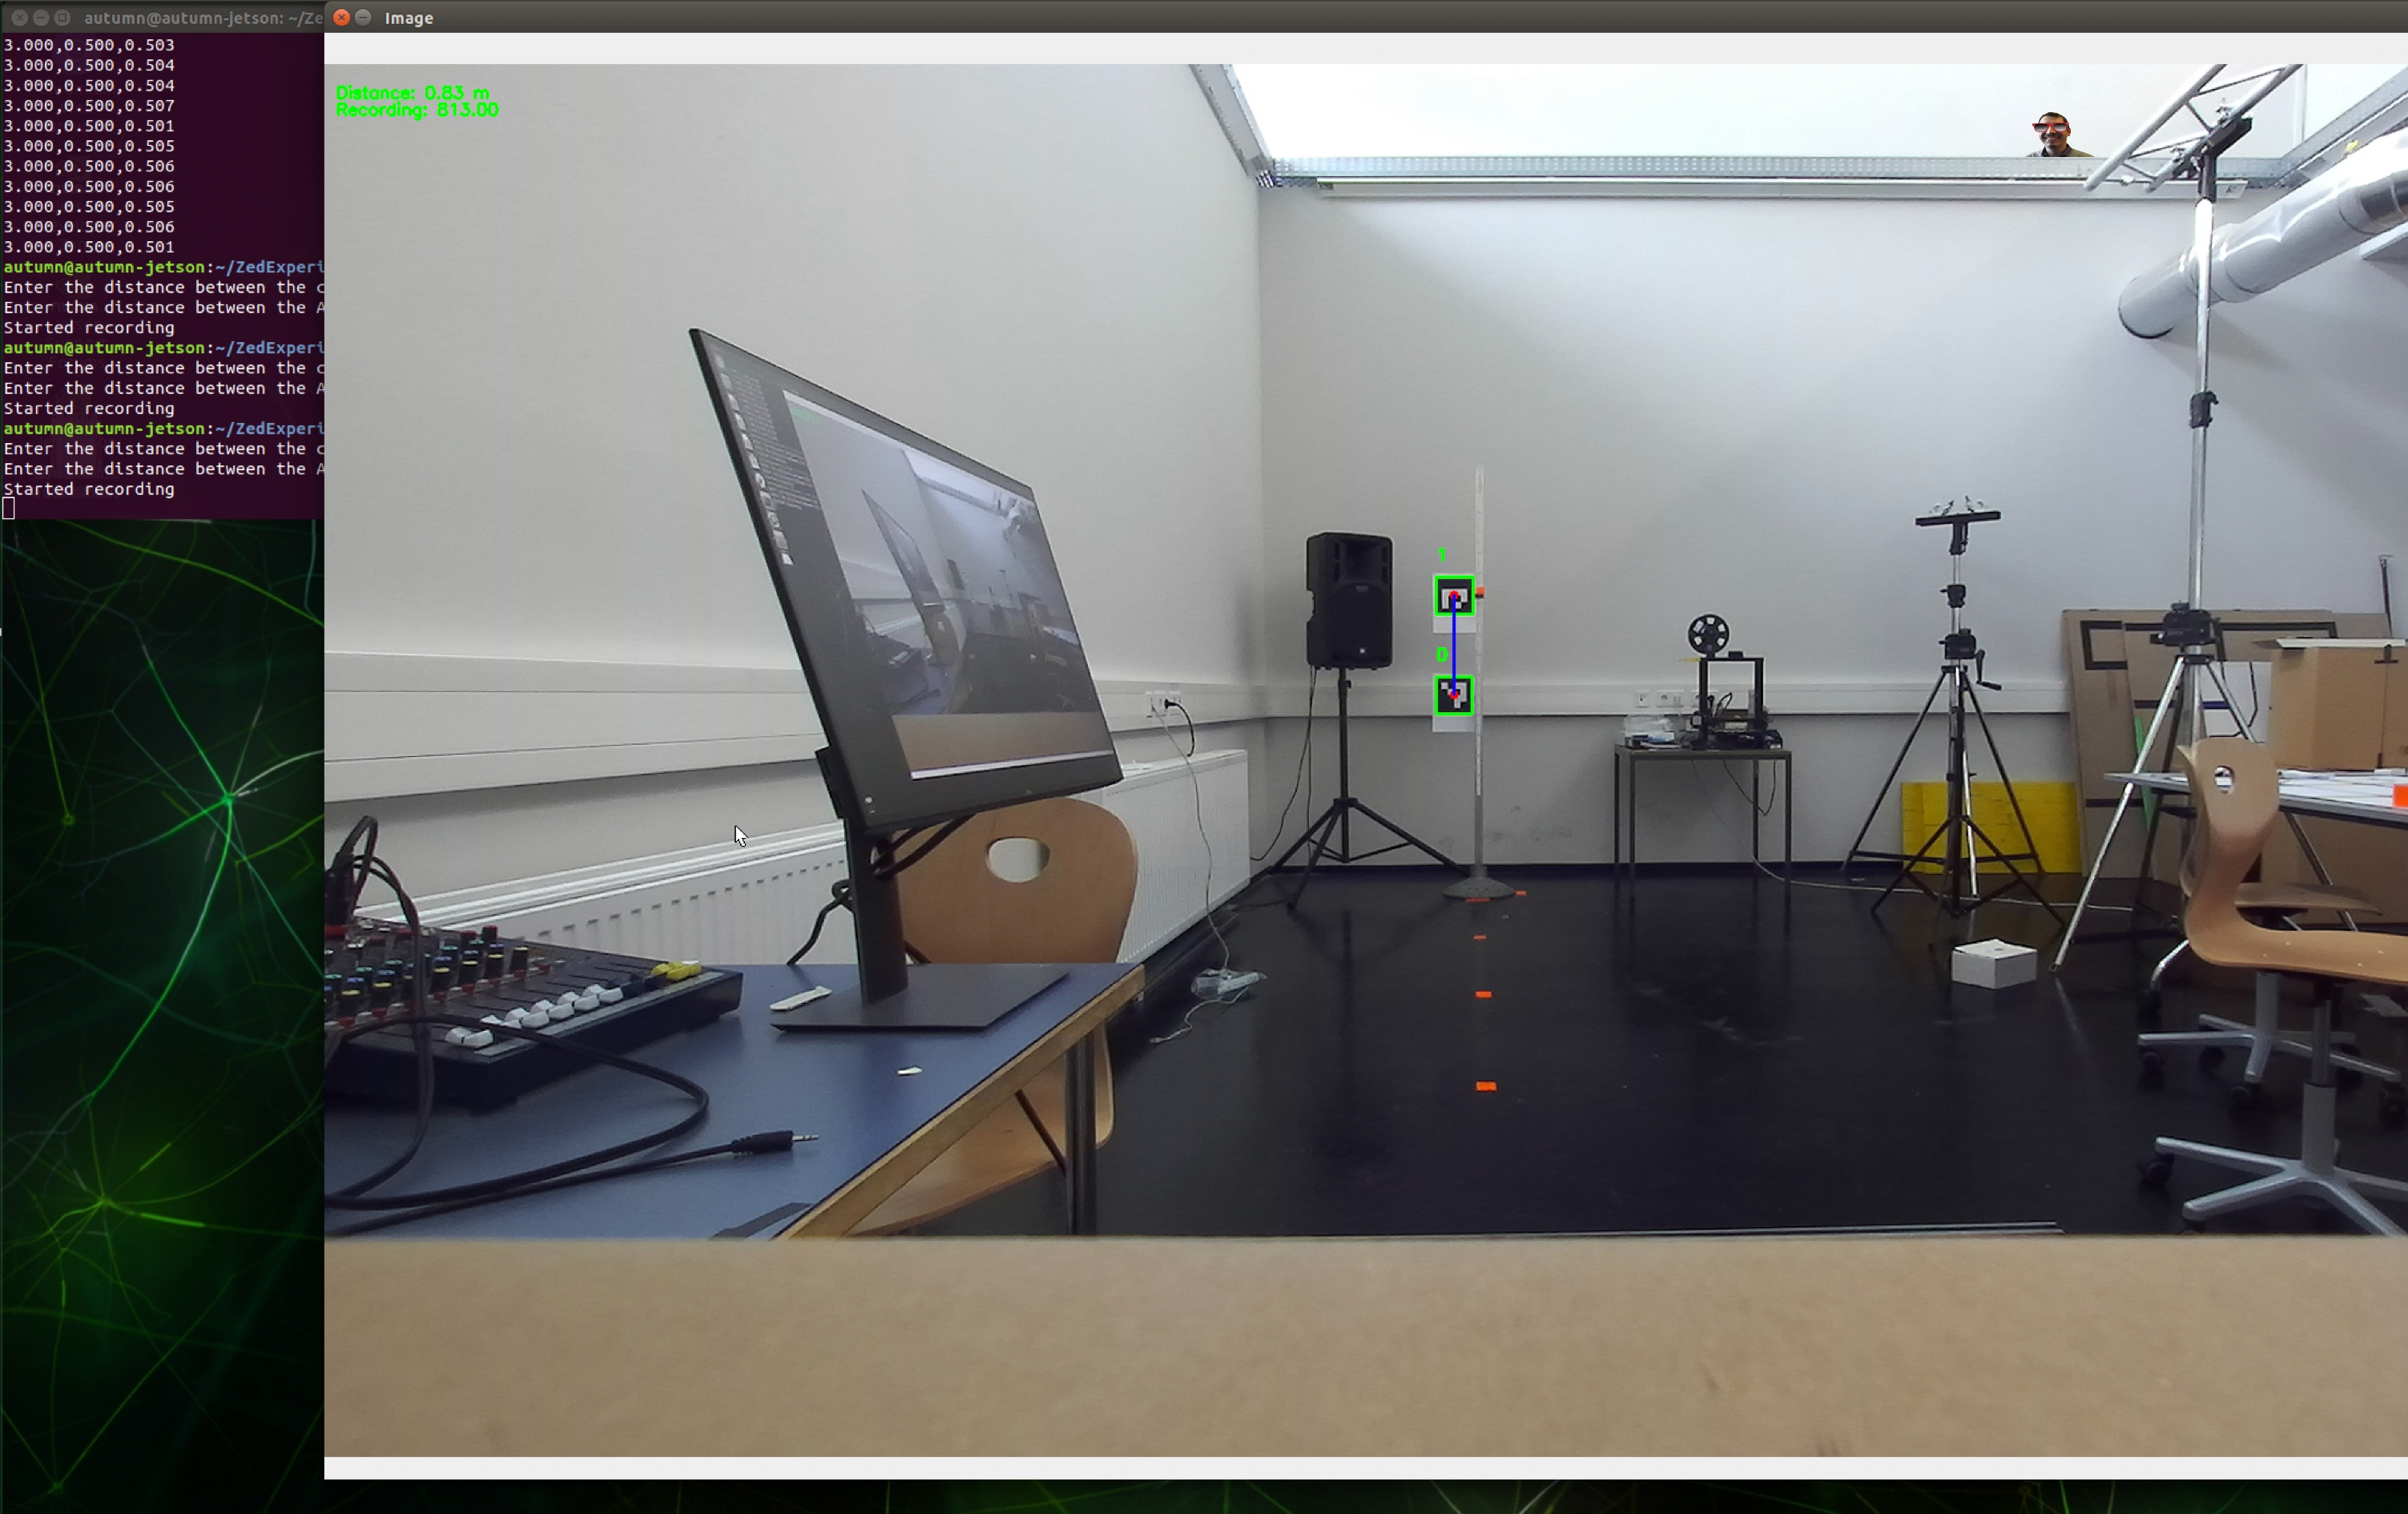
\includegraphics[width=0.8\linewidth]{img/AutumnZEDBenchmark}
	\caption{
		Picture of how the distance between to ARUCO tags was measured in the experimental setting.
	}
	\label{fig:zedExperiment}
\end{figure}

To answer this question the cameras measured the vertical distance enclosed by two points mounted 1 m above each other on a stationary structure, with the bottom one at a height 1 m above the ground. 
The cameras were placed on a movable rig perpendicular to the stationary structure and 1m above the ground. The cameras measured the aforementioned gap at 1 m increments between 3 m and 10 m horizontal distance measured amongst each structure's base. 

The usage of ARUCO tags allowed for precisely tracking the position of each point within the camera coordinate system, thus ensuring the points remain fixed even though the camera rig is moved. This is visible in Figure \ref{fig:zedExperiment}
% über ARUCO schreiben
% reference zu ARUCO 
ARUCO tags are square-based markers popular in many robotic and augmented reality applications. They provide a fast and robust solution for estimating a camera's pose relative to one or multiple markers. Each marker has a unique, identifiable pattern that allows for precisely determines and tracks its position.\footcite{jurado2015} 

\subsubsection{Results - ZED1}

Figure \ref{plot:zed1Benchmark} depicts the mean, minimal and maximal depth-perception error measured, thus indicating how well the camera performed.
To illustrate the underlying model of this data, a cubic regression is superimposed. This well-fitted model indicates a relatively steady error just under 0.1 m which increases drastically after a local minimum at a distance of 5.6 m. 
While the mean error increases, the minimal deviation declines to 0 m between distances of 6 m to 8 m, indicating an optimal interval for measurements. Although the maximal error thrives within this range, it generally remains close to the mean at all other distances.
Table \ref{tab:resultsZed1} shows the data these findings are based on as well as a total mean, minimal and maximal deviation over all distances. 
In total, the ZED 1 has a mean error of 13\%, which is drastically above what the cameras data sheet states\footcite{zed1Datasheet}.

%
%The mean depth-perception error dependant on the camera distance for the ZED 1 (blue) is plotted in Fig. \ref{plot:zedBenchmark}. To illustrate the positive tendency a linear regression (cyan) is superimposed. The trend line indicates a relatively steep slope with the mean error adding up by 0.03 m at increasing distances from the rig. Additionally the error range listed in Tab. \ref{tab:errorMinimaMaxima} shows a base error of 0.7\% and a maximum mean error of 3\%, which is similar to the error stated by the cameras data sheet\footcite{zed1Datasheet}.
%
%The data for the ZED 2 (red) and its corresponding trend line (orange) indicate a much more shallow slope with 0.01 m per meter distance to the rig. Looking at the error range the ZED 2 lies below 1\% mean error at all distances which also corresponds to the data sheets specifications \footcite{zed2Datasheet}.


%When comparing each trend line for each camera it is apparent that the slope of the ZED 1 with $0.03m/m$ is more than twice as large compared to the ZED 2 at $0.01m/m$. This indicates that with increasing distance the depth-perception error increases dramatically. 
%Another interesting finding are the minima and maxima of the mean depth-perception error found in Tab. \ref{tab:errorMinimaMaxima}.
%As illustrated the ZED 1 inherits a substantially large minimal and maximal error of  $0.07m$ and $0.31m$.
%Compared to this the ZED 2 performed much better with a almost non existent base error and a maximal error of $0.1m$.

%\begin{table}[h]
%	\centering
%	\begin{tabular}{|l|l|l|}
%		\hline
%		& \textbf{Minimal Mean Error} & \textbf{Maximal Mean Error} \\ \hline
%		\textbf{ZED 1}  & 0.07 m 					  & 0.31 m                      \\ \hline
%		\textbf{ZED 2} & 0.01 m                      & 0.10 m                      \\ \hline
%	\end{tabular}
%	\caption{Table containing the minimal and maximal mean error of both the ZED 1 and ZED 2.}
%	\label{tab:errorMinimaMaxima}
%\end{table}

\begin{table}[h]
	\centering
	\begin{tabular}{|l|l|l|l|l|l|l|l|l|l|}
		\hline
		\textbf{Distances {[}m{]}}      & 3    & 4    & 5    & 6    & 7    & 8    & 9    & 10   & {\ul Total} \\ \hline
		\textbf{Mean Deviation {[}m{]}} & 0.07 & 0.08 & 0.09 & 0.08 & 0.09 & 0.14 & 0.17 & 0.31 & {\ul 0.13}  \\ \hline
		\textbf{Min Deviation {[}m{]}}  & 0.07 & 0.04 & 0.04 & 0.00 & 0.00 & 0.00 & 0.01 & 0.01 & {\ul 0.00}  \\ \hline
		\textbf{Max Deviation {[}m{]}}  & 0.08 & 0.11 & 0.13 & 0.45 & 0.67 & 0.18 & 0.24 & 0.84 & {\ul 0.84}  \\ \hline
	\end{tabular}
	\caption{Summarized data of mean, minimal and maximal deviation for the ZED 1 camera at increasing distances.}
	\label{tab:resultsZed1}
\end{table}

\begin{figure}[h]
	\begin{center}
		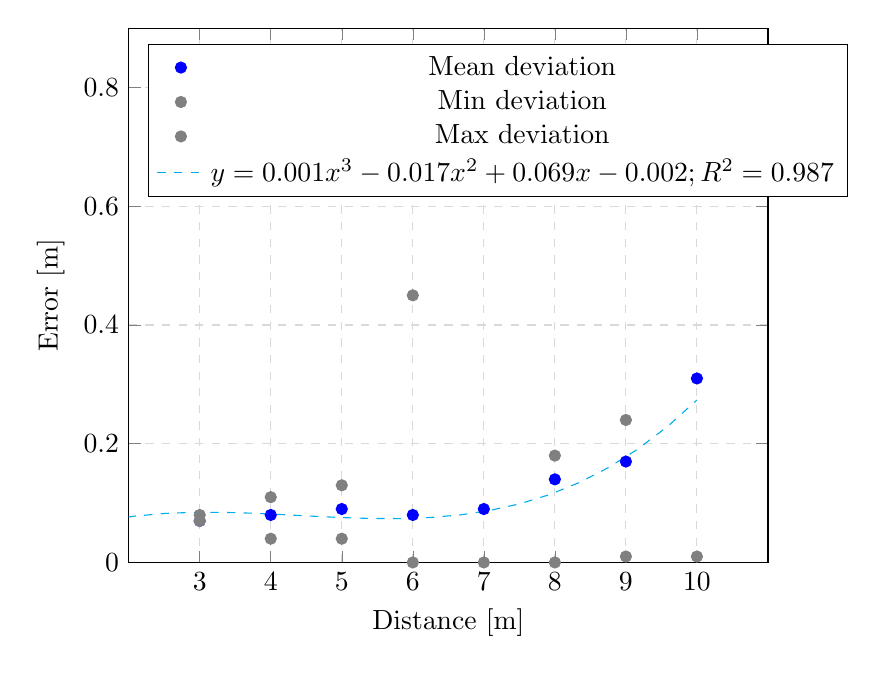
\begin{tikzpicture}
			\begin{axis}[
				width=0.8\linewidth, % Scale the plot to \linewidth
				grid=major, 
				grid style={dashed,gray!30},
				xlabel={Distance [m]}, % Set the labels
				ylabel={Error [m]},
				legend pos=north west,
				xtick={3, 4, 5, 6, 7, 8, 9, 10},
				xmin=2,
				xmax=11,
				ymin=0,
				ymax=0.9,
				]
				
				
				%zed1 mean
				\addplot[only marks, color=blue]
				table[row sep=crcr]{
					distance error \\
					0 0 \\
					3 0.07 \\
					4 0.08 \\
					5 0.09 \\
					6 0.08 \\
					7 0.09 \\
					8 0.14 \\
					9 0.17 \\
					10 0.31 \\
				}; 
				\addlegendentry{Mean deviation}
				
				%zed1 min
				\addplot[only marks, color=gray]
				table[row sep=crcr]{
					distance error \\
					0 0 \\
					3 0.07 \\
					4 0.04 \\
					5 0.04 \\
					6 0 \\
					7 0 \\
					8 0 \\
					9 0.01 \\
					10 0.01 \\
				}; 
				\addlegendentry{Min deviation}
				
				%zed1 max
				\addplot[only marks, color=gray]
				table[row sep=crcr]{
					distance error \\
					0 0 \\
					3 0.08 \\
					4 0.11 \\
					5 0.13 \\
					6 0.45 \\
					7 0.67 \\
					8 0.18 \\
					9 0.24 \\
					10 0.84 \\
				}; 
				\addlegendentry{Max deviation}
				
				%zed1 mean regression
%				\addplot[no marks, color=orange, style=dashed]
%				table[row sep=crcr, y={create col/cubic regression={y=error}}]{
%					distance error \\
%					0 0 \\
%					3 0.07 \\
%					4 0.08 \\
%					5 0.09 \\
%					6 0.08 \\
%					7 0.09 \\
%					8 0.14 \\
%					9 0.17 \\
%					10 0.31 \\
%				};
				\addplot[no marks, color=cyan, style=dashed, domain=0:10] (x, 0.0013*x*x*x - 0.0171*x*x + 0.0686*x - 0.0024);
				\addlegendentry{$y = 0.001x^3 - 0.017x^2 + 0.069x - 0.002; R^2 =  0.987$} 
				
			\end{axis}
		\end{tikzpicture}
		\caption{This plot describes how the mean (blue), as well as minimal and maximal (grey) depth-performance error of the ZED 1 Stereo Camera changes with increasing distance to an object. Furthermore the cubic regression function (cyan) for this data is plotted. 
		 }
	 	\label{plot:zed1Benchmark}
	\end{center}
\end{figure}



\subsubsection{Results - ZED 2i}

Data for the mean, minimal and maximal depth-perception error of the ZED 2i is plotted in Figure \ref{plot:zed2Benchmark}.
%The cubic regression model for this camera indicates a coherently low mean error which decreases after a local maximum at a distance of 8.6 m. 
The cubic regression model for this camera indicates a slight negative trend with a coherently low mean error, peaking at a local maximum at 8.6 m. However, the initial belief suggests that with increasing distances, the error thrives correspondingly. According to the coefficient of determination $R^{2}$, indicating that the cubic regression function does not fully match the data, a different regression model may result in more accurate assertions supporting the initial belief. 
Considering the overall error range, the minimal error remains below 0.02 m for all distances while the maximal error grows to approximately 0.4 m. 
An optimal measurement zone due to moderate mean and non-existent minimal deviation can be observed between 7 m and 8 m. 
Table \ref{tab:resultsZed2} indicates an overall mean error of 5\%, which does correspond to the statement of the ZED 2i data sheet\footcite{zed2Datasheet}.



\begin{table}[h]
	\centering
	\begin{tabular}{|l|l|l|l|l|l|l|l|l|l|}
		\hline
		\textbf{Distances {[}m{]}}      & 3    & 4    & 5    & 6    & 7    & 8    & 9    & 10   & {\ul Total} \\ \hline
		\textbf{Mean Deviation {[}m{]}} & 0.01 & 0.01 & 0.06 & 0.08 & 0.05 & 0.04 & 0.10 & 0.08 & {\ul 0.05}  \\ \hline
		\textbf{Min Deviation {[}m{]}}  & 0.00 & 0.00 & 0.01 & 0.02 & 0.00 & 0.00 & 0.02 & 0.02 & {\ul 0.00}  \\ \hline
		\textbf{Max Deviation {[}m{]}}  & 0.03 & 0.11 & 0.26 & 0.24 & 0.42 & 0.35 & 0.43 & 0.41 & {\ul 0.43}  \\ \hline
	\end{tabular}
	\caption{The mean, minimal and maximal depth-perception deviation measured by the ZED 2i.}
	\label{tab:resultsZed2}
\end{table}

\begin{figure}[h]
	\begin{center}
		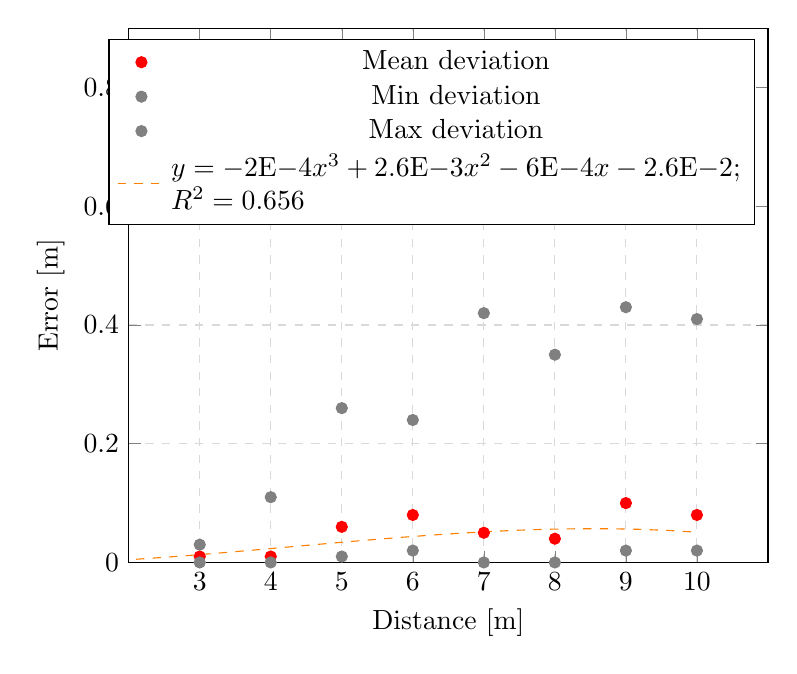
\begin{tikzpicture}
			\begin{axis}[
				width=0.8\linewidth, % Scale the plot to \linewidth
				grid=major, 
				grid style={dashed,gray!30},
				xlabel={Distance [m]}, % Set the labels
				ylabel={Error [m]},
				legend style={cells={align=left}},
				xtick={3, 4, 5, 6, 7, 8, 9, 10},
				xmin=2,
				xmax=11,
				ymin=0,
				ymax=0.9,
				]
				
				
				%zed2 mean
				\addplot[only marks, color=red]
				table[row sep=crcr]{
					distance error \\
					0 0 \\
					3 0.01 \\
					4 0.01 \\
					5 0.06 \\
					6 0.08 \\
					7 0.05 \\
					8 0.04 \\
					9 0.10 \\
					10 0.08 \\
				}; 
				\addlegendentry{Mean deviation}
				
				%zed2 min
				\addplot[only marks, color=gray]
				table[row sep=crcr]{
					distance error \\
					0 0 \\
					3 0. \\
					4 0 \\
					5 0.01 \\
					6 0.02 \\
					7 0 \\
					8 0 \\
					9 0.02 \\
					10 0.02 \\
				}; 
				\addlegendentry{Min deviation}
				
				%zed2 max
				\addplot[only marks, color=gray]
				table[row sep=crcr]{
					distance error \\
					0 0 \\
					3 0.03 \\
					4 0.11 \\
					5 0.26 \\
					6 0.24 \\
					7 0.42 \\
					8 0.35 \\
					9 0.43 \\
					10 0.41 \\
				}; 
				\addlegendentry{Max deviation}
				
				%zed2 mean regression
%				\addplot[no marks, color=cyan, style=dashed]
%				table[row sep=crcr, y={create col/cubic regression={y=error}}]{
%					distance error \\
%					0 0 \\
%					3 0.01 \\
%					4 0.01 \\
%					5 0.06 \\
%					6 0.08 \\
%					7 0.05 \\
%					8 0.04 \\
%					9 0.10 \\
%					10 0.08 \\
%				};
				\addplot[no marks, color=orange, style=dashed, domain=0:10] (x, -0.0002*x*x*x + 0.0026*x*x - 0.0006*x - 0.003);
				\addlegendentry{$y = -2\mathrm{E}{-4} x^3 + 2.6\mathrm{E}{-3} x^2 - 6\mathrm{E}{-4} x - 2.6\mathrm{E}{-2};$ \\ $R^2 =  0.656$} 
				
			\end{axis}
		\end{tikzpicture}
		\caption{
			This plot describes how increasing distances to a stationary object affect the mean (red), as well as minimal and maximal (grey) depth-performance error of the ZED 2i. The model describing this data is approximated using a cubic regression (orange).
		}
		\label{plot:zed2Benchmark}
	\end{center}
\end{figure}



\subsubsection{Comparison}

Comparing both models, the ZED 1 clearly shows a much more aggressive upwards trend than the ZED 2i, which has a relatively monotonic mean error. 

However, both cameras share a commonly low minimal error indicating that both can correctly and precisely take depth measurements within the tested distances. 
Although the ZED 2i generally outperforms its predecessor concerning mean deviation, its maximal depth-perception error strays drastically further from the mean compared to the ZED 1. 


%Comparing both trend lines and mean error range the ZED 1 clearly shows a much more aggressive upwards trend and higher base error compared to the ZED 2. However as the coefficient of determination $R^{2}$ for each trend line indicate a mediocre fit the aforementioned assumptions should not be solely taken into consideration when comparing the two camera systems. 

Having said this, in combination with the data sheets, the overall trend on depth-performance meets the initial assumption and justifies the upgrade to the ZED 2i.

%Considering all of the aforementioned findings it is apparent that the ZED 2 produced much better depth-perception results compared to the ZED 1. This justifies the upgrade not only from a feature focused standpoint but also quality wise as this greatly effects the final 3D point cloud utilized by components discussed later in this thesis. 

\filbreak